\chapter{Introduction}

\section{Surgical robotics}

\subsection{Historical Overview of Surgical robotics}

In surgical robotics, the surgeon operates on the patient using a computer-controlled robotic arm, to which the surgical tools needed for the operation are attached. According to surgical bibliography, robotics and laparoscopic procedures are used in general surgery, cardiothoracic surgeries, colon surgeries, gynecology, neurosurgery and orthopedics. 

Robotic mechanisms were first introduced in Medicine, in 1987 with the first laparoscopic surgery of a cholecystectomy followed by several laparoscopic operations. Such surgical operations are characterised as \textbf{minimally invasive}, because the surgical incisions made at the patient are very small leading to a small probability of infection of the patient. a reduction of the hospitalization time and an overall faster patient recovery. 

However, traditional laparoscopic mechanisms have some downsides as well. First of all, the surgeon should operate in a mirrored-way, meaning that they should move at the opposite direction from what they saw at the screen (this effect is also known as the \textbf{fulcrum effect}), in order to reach the desired point of operation. Earlier laparoscopic tools had less degrees of freedom, which means less flexibility in motion control. Moreover these systems provided limited touch sensibility and feedback to the doctor while being very susceptible to the surgeon's micro movements and tremble. 

The first application of robotics in surgery appears in 1985, when Kwoh et al. \cite{Shao1985ANC} used a \textbf{PUMA 560}, a standard industrial robotic arm, to perform a neurosurgical biopsy, where the biopsy needle was inserted in the brain and guided with the help of Computed Tomography. This successful application was followed by the \textbf{PROBOT} surgical robot \cite{Probot1992}, which was developed at the Imperial College and used in a prostatectomy operation. Another example of an early surgery robot was the \textbf{ROBODOC} system \cite{Robodoc} developed by Integrated Surgical Supplies in Sacramento California, which was the first to be used in orthopedics for a hip replacement surgery and was also the first to be approved by the FDA (Food \& Drug Administration).

\begin{center}
\begin{figure}[!htb]
\centering
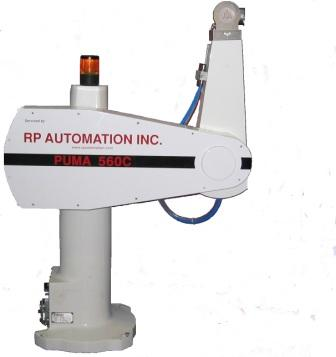
\includegraphics{images/Puma560.jpg}\\
\caption{First Surgical Robot PUMA 560 (circa 1985)}
\end{figure}
\end{center}

Some other important surgery robots are listed in the sequel:
\begin{itemize}
\item \textbf{AESOP\textsuperscript \textregistered Endoscope Positioner}: A voice controlled endoscopic system
\item \textbf{HERMES\textsuperscript \textregistered Control Center}
\item \textbf{daVinci Surgical System\textsuperscript \textregistered}: The  most popular surgery robots in a master-slave configuration, implying that the operation commands are sent uni-directionally from the master console, which is controlled by the surgeon, and are executed by the robot. It also comes with a high definition 3D video feed and advanced tooling system, one for each hand, called EndoWrist\textsuperscript \textregistered. It is officially approved 
by the FDA for laparoscopic surgeries.
\item \textbf{SOCRATES Robotic Telecollaboration System}
\item \textbf{Raven-II} \cite{Raven2}: An open platform for collaborative research on surgical robotics.
\item \textbf{Monarch\textsuperscript \texttrademark Platform} by Auris Health Inc., an endoscopic system for robotic-assisted bronchoscopy
\end{itemize}

\begin{center}
\begin{figure}[htbp]
\centering
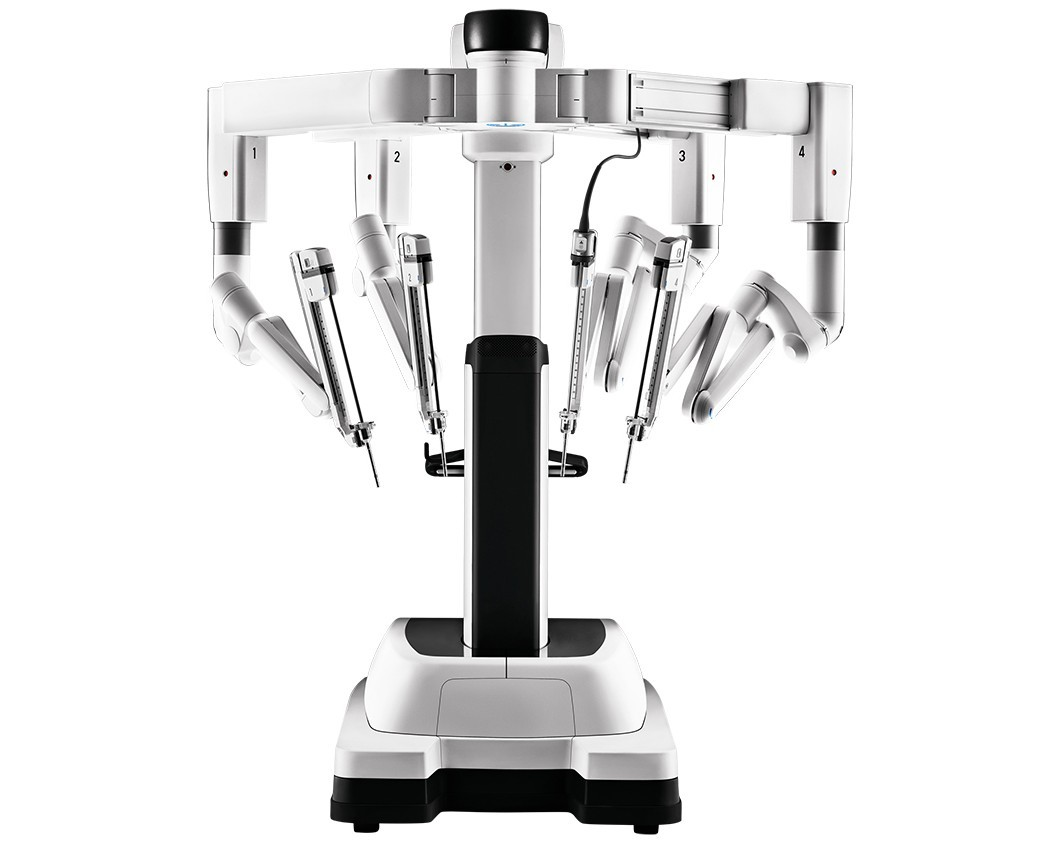
\includegraphics[width=0.7\textwidth]{images/intuitive-da-vinci-xi-patient-cart-front-view-1060867-lo-res.jpg}\\
\caption{DaVinci Xi, \textsuperscript \textcopyright 2020 Intuitive Surgical, Inc. Patient Cart with the robotic arms that control the surgical tools}
\end{figure}
\end{center}

\begin{center}
\begin{figure}[htbp]
\centering
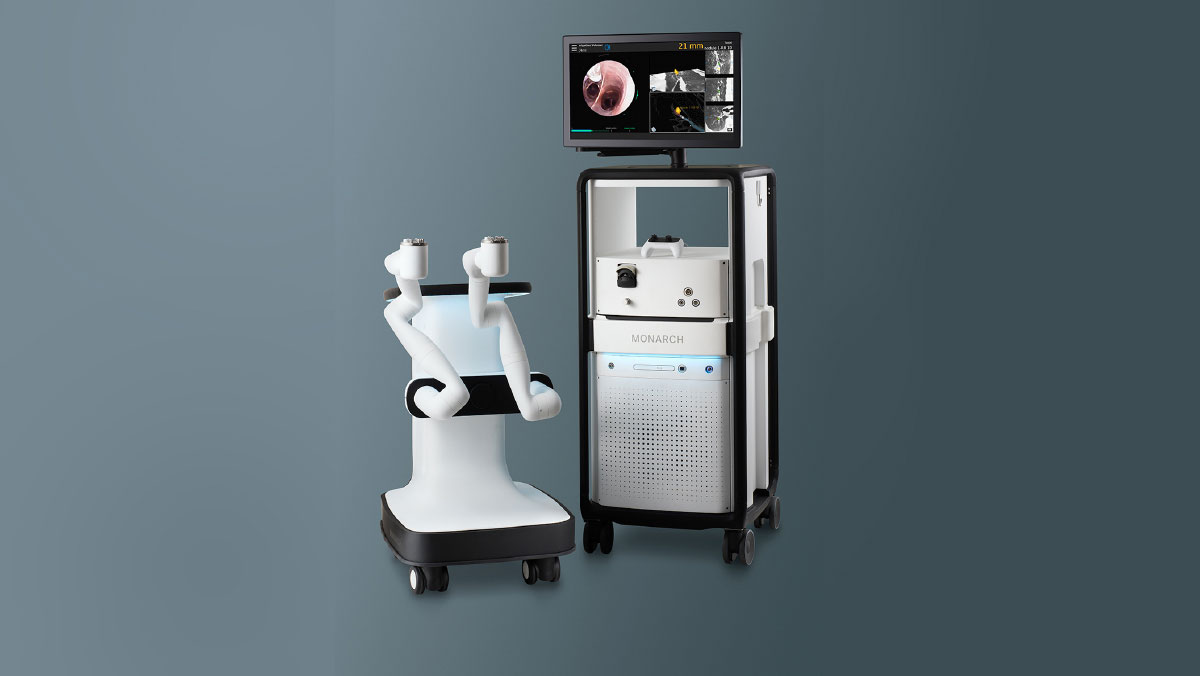
\includegraphics[width=0.8\textwidth]{images/Moarch_Platform_1200_x_676_1_.jpg}\\
\caption[The Monarch\textsuperscript \texttrademark Platform endoscopic system]{The Monarch\textsuperscript \texttrademark Platform endoscopic system \footnotemark}
\end{figure}
\end{center}
% How to use caption with footnote https://tex.stackexchange.com/questions/10181/using-footnote-in-a-figures-caption 
\footnotetext{\url{https://www.aurishealth.com/patients/robotic-bronchoscopy-patient-about-monarch-platform }}


\subsection{Surgical Robotic Procedure}

The robotic surgery procedure starts with total anesthesia of the patient. Then the surgeon makes small incisions at the anatomical region of interest, where the procedure will take place. Through these small incisions special tubes, called trocars are mounted followed by an insertion of the laparoscopic tools. After the patient is prepared and after the patient cart, which carries the robotic arms, is successfully positioned and callibrated, the surgeon sits on a console, from where he/she controls the robot via special sensitive joysticks. The surgeon has 3D-visual access to the surgical site via a small endoscopic camera and the video is displayed on the console. In some cases, the surgeon gets force feedback from the joysticks via haptic mechanisms. Haptic force feedback is very important for the doctor in order to have a better sense of the anatomy and the surgical site, and it has gained a lot of interest in the research community.

\begin{center}
\begin{figure}[htbp]
\centering
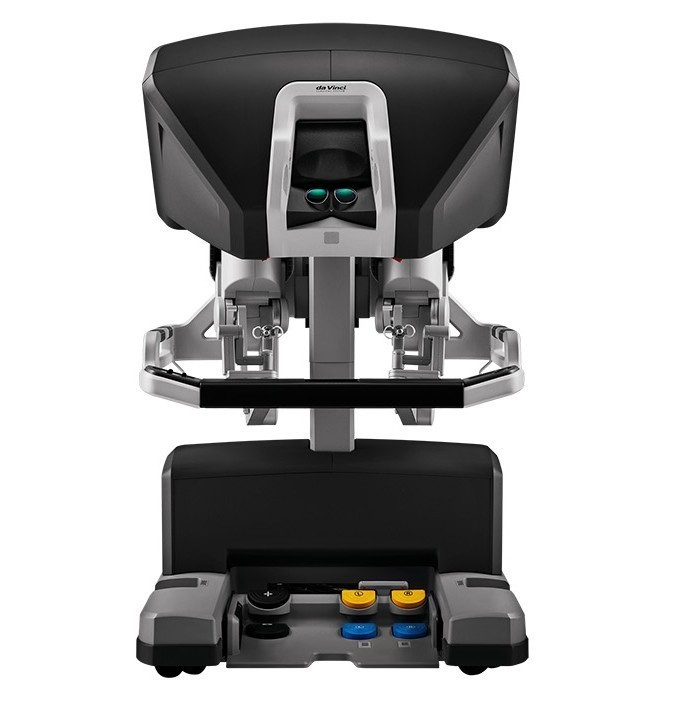
\includegraphics[width=0.5\textwidth]{images/intuitive-davinci-console-front-lowres.jpg}\\
\caption[DaVinci Xi \textsuperscript \textcopyright 2020 Intuitive Surgical, Inc. Surgeon Console]{DaVinci Xi \textsuperscript \textcopyright 2020 Intuitive Surgical, Inc. Surgeon Console \footnotemark}
\end{figure}
\end{center}
\footnotetext{\url{https://www.intuitive.com/en-us/about-us/press/press-resources}}

%
%\subsection{Advantages \& Disadvantages of Surgical robotics}
%
The advantages offered by Surgical robotics include but not limited to:
\begin{itemize}
\item \textbf{Minimally Invasive Procedures} which means
	\begin{itemize}
	\item Smaller incisions
	\item Less blood loss
	\item Reduced risk of inpatient infection
	\item Less pain
	\item Faster patient recovery
	\end{itemize}
\item Increased \textbf{precision} and reduced human errors
	\begin{itemize}
	\item Smooth and precise movements
	\item Detection and correction of errors caused by hand tremble
	\end{itemize}
\item \textbf{No fulcrum effect} and intuitive manipulation of surgical tools
\item \textbf{Haptic feedback}. This technology uses small mechanical forces and vibrations to give the user the sense of touch or force. Force feedback gives the ability to the surgeon to understand the mechanical properties of the tissue they operate on, such as resistance and elasticity, and thus distinguish between healthy from unhealthy tissue
\item \textbf{Teleoperation}: the surgeon operates while he/she sits on a special \textbf{ergonomic} console, which makes the long procedures more comfortable and efficient.
\end{itemize} 

\section{Thesis Strategic Goals}

The goal of this thesis is to design the kinematic models and algorithms necessary for a robotic arm to detect, grasp and manipulate a laparoscopic surgical tool. To achieve these goals the robotic arm should be capable of the following:
\begin{itemize}
\item Visually detect the scene and laparoscopic tools and with the help of stereoscopic vision, and calculate the relative position and orientation of the center of mass of each tool
\item Calculate the contact points on the tool, on which the fingers of the gripper will be placed, so that there is a firm grasp (force closure)
\item Calculate the path from the tools' table to the surgical site table
\item Calculate the trajectory that needs to be executed when the tool is inserted in the trocar. This is a special type of trajectory, because the motion is constrained and is known in the bibliography as RCM-control. The constraint is that, at each time one point of the inserted tool must coincide with the RCM point (this point will also be referenced in this thesis as the center of the 
trocar, or the fulcrum reference frame point).
\end{itemize}

%
\section{Related Past Overview}

Surgery robotics, in terms of robot mechanics, can be divided into two categories, specialized surgical robots and generic robotic arms that are programmed for surgical tasks. The specialized surgical robots have specific mechanisms which ensure that the RCM constraint is satisfied mechanically. These robots are easier to control but are only suitable for very specific operations and are usually large in size, with complicated structures that require more maintenance.

A new methodology to perform MIS-procedures is by using industrial robots which are programmable to respect the RCM constraint. This methodology is studied in \cite{Marinho2014APR}, where a controller is designed to minimize the deviation from the RCM point using kinematics with the dual quaternion framework. A similar approach is studied in \cite{Bauzano2009ControlMF}, where a controller is designed for an active wrist robot to mimic the passive wrist mechanism, which means not exerting pressure on the abdominal wall and respecting the RCM constraint while executing the trajectory with smaller error.

This thesis follows a similar approach, where the laparoscopic tool is attached on an active wrist end-effector of a popular non-surgical industrial robot (KUKA lwr iiwa14) and the RCM constraint is satisfied with non specialized mechanisms or a passive wrist.

Minimizing the RCM error is important in order to execute precise trajectories but also to minimize the force exerted to the patient. In~\cite{4957177}, this deviation error is studied more thoroughly and is used to study the 
force interaction model of the surgical tool (endoscopic camera) and the abdominal wall. The force that is exerted can be calculated from the fulcrum displacement and the abdominal wall elasticity constant which can be 
estimated experimentally.

The trajectories that a laparoscopic tool must follow, pivot around the RCM constraint point. This point is also known in the bibliography as the fulcrum point, pivot point, trocar point, and incision point. To design a 
trajectory, this point is assumed to be known within some bounds. In~\cite{Dong2016RobustTD} an algorithm is proposed that estimates the position of the trocar during a robot-assisted endoscopic surgery. The trocar position is estimated with the Least Squares algorithm which is used to calculate the intersection of surgical tool axes measured from a given number of consecutive robot configurations. A different approach of estimating the Fulcrum point is presented in~\cite{Gruijthuijsen2018LeveragingTF}, where the fulcrum point is estimated using an Extended Kalman FIlter which uses a stochastic measurement and prediction model and it is able to produce adeqiuate results in the presence of noise.

When designing a control system for the robot, capable of executing the pivot motions, there are two approaches. The first approach is to directly design a control system whose control parameters adapt to the errors (direct 
adaptive control) and the second approach is to initially estimate the fulcrum parameters or assume they are known and then apply a usual control system (indirect adaptive control). An example of the second approach is studied in 
\cite{Muoz2005PivotingMC}, where a geometrical estimator is used to estimate the outside penetration of the surgical tool, which is then used in a PI controller and a trajectory generator.

\section{Adopted Methodology \& Approach}

In designing a robotic arm to execute a surgery task, there is a need to subdivide the task in multiple smaller submodules and design, implement and test each submodule separately and then combine them together for end-to-end testing.

\begin{center}
\begin{figure}[!htb]
\centering
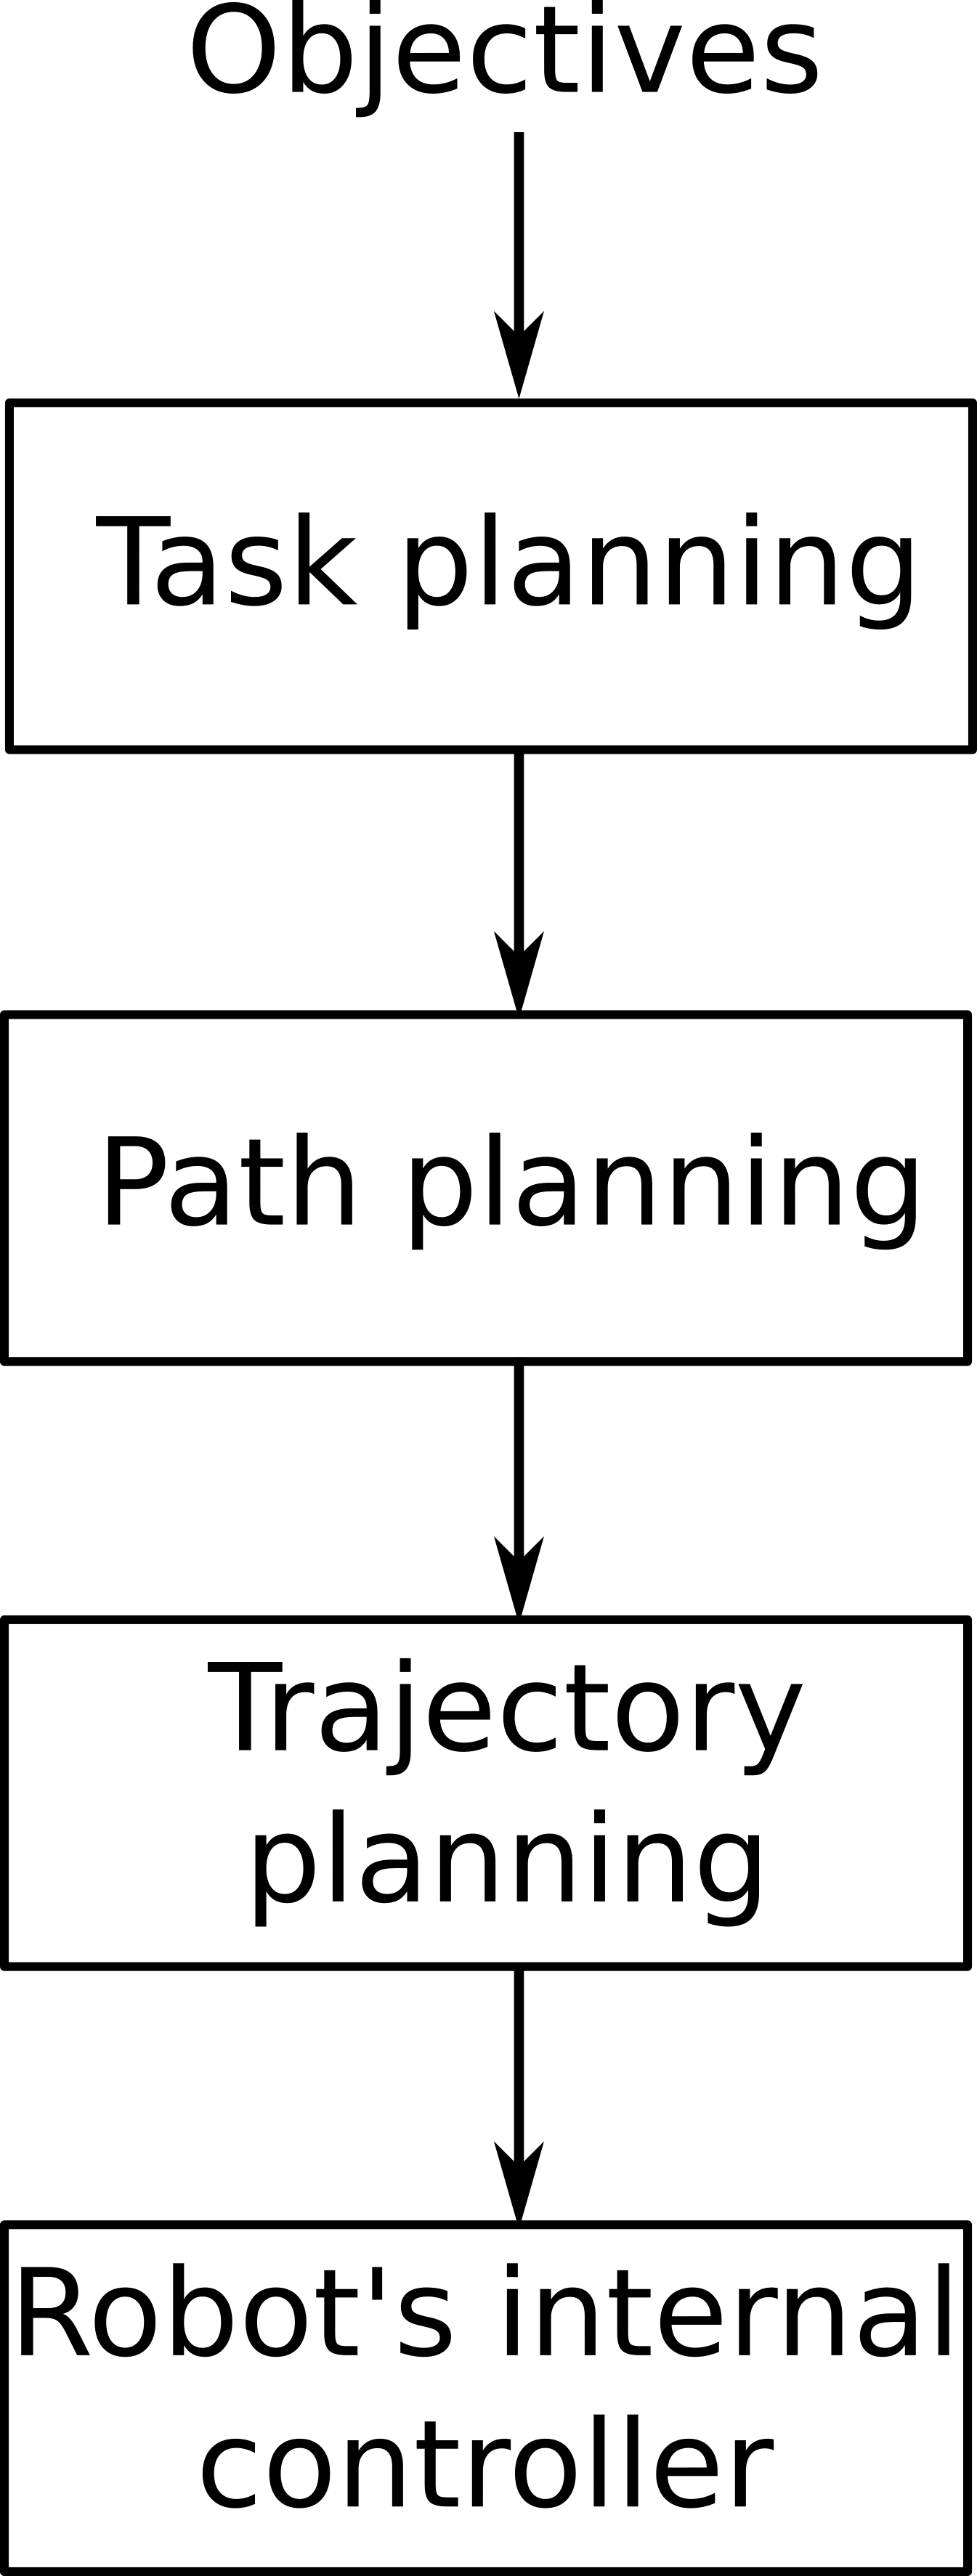
\includegraphics[width=0.15\textwidth]{images/motion-planning.png}\\
\caption{Motion planning pipeline}
\end{figure}
\end{center}

\textbf{Tools \& Software used in this thesis}:
\begin{itemize}
\item Matlab \& Matlab toolboxes: ROS Toolbox, Robotics Toolbox
\item ROS Framework
\item MoveIt
\item Gazebo simulator
\item VREP simulator
\item OpenCV
\end{itemize}

\textbf{Methodology of conducting this thesis}:
\begin{itemize}
\item Mathematical calculations for Kinematics and Motion planning
\item Mathematics validation with Matlab
\item Quick prototyping and testing with Matlab and/or VREP
\item Implementation in ROS frameworks, by splitting the end-to-end robotic operation in smaller experiments and tasks
\end{itemize}

\begin{center}
\begin{figure}[htbp]
\centering
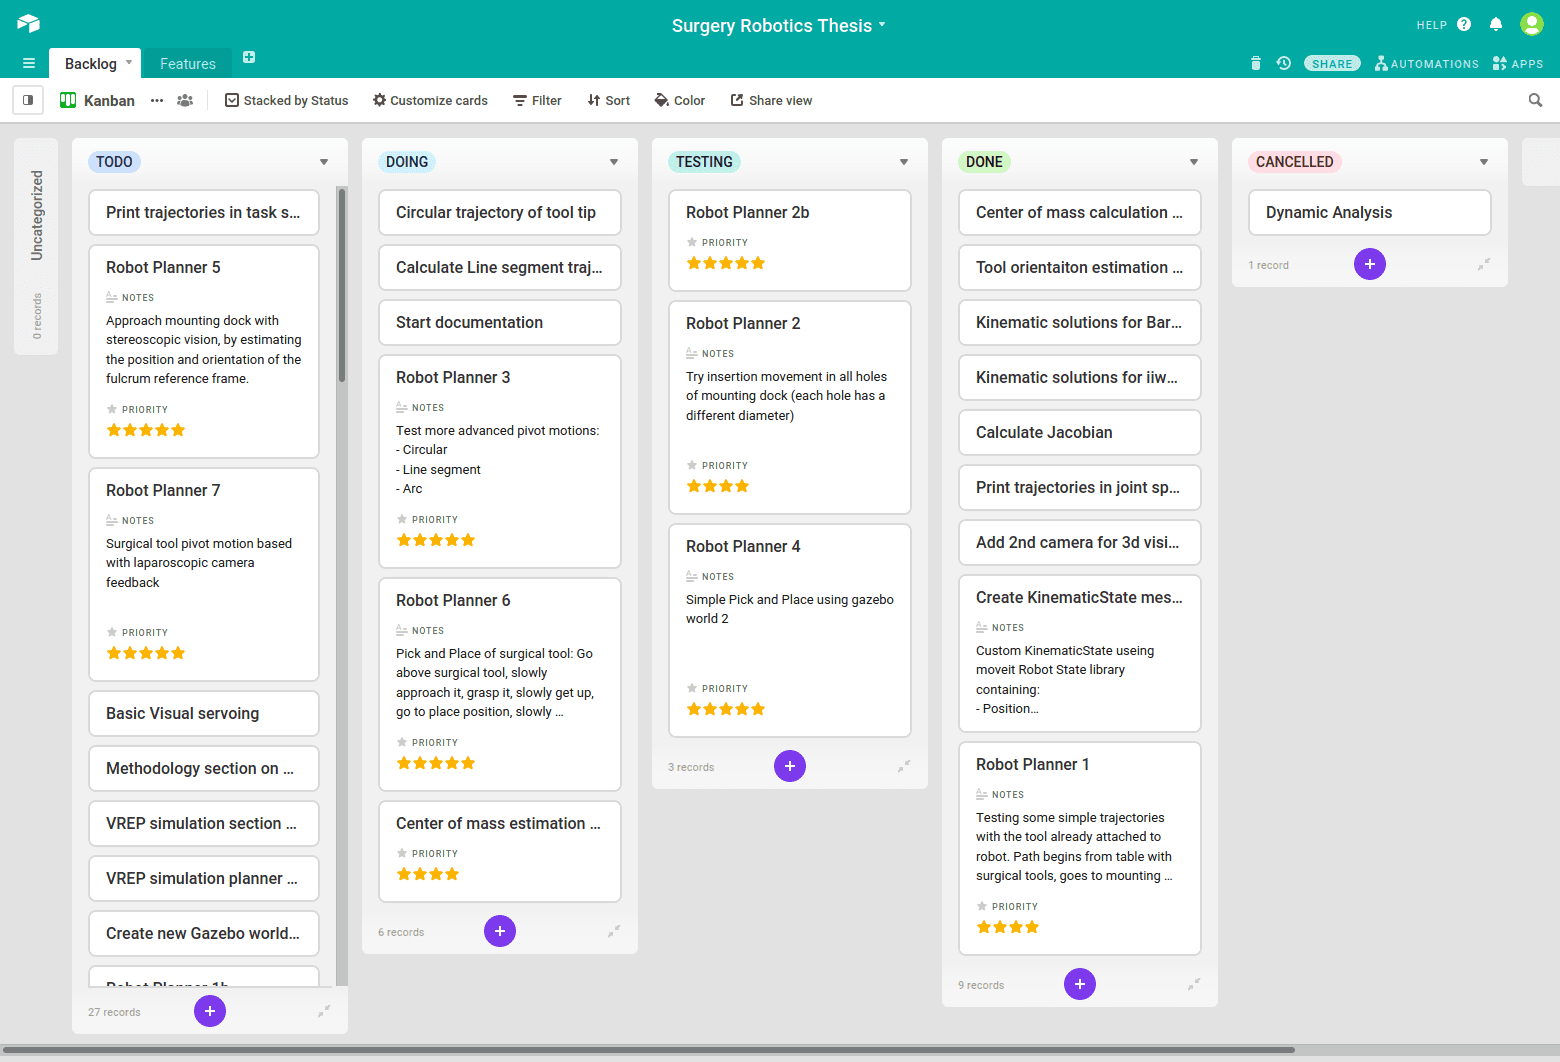
\includegraphics[width=0.7\textwidth]{images/task-backlog-airtable.png}\\
\caption{Kanban view of backlog tasks to organize all features, requirements and tasks needed to complete this thesis. The tool used to keep track of all tasks is Airtable}
\end{figure}
\end{center}

To quickly test out ideas on how to build the robot's environment and the simulation layout, as well as some simple trajectories, the CoppeliaSim simulator software was used (also known previously as VREP). CoppeliaSim allowed to do quick prototyping using the intuitive drag-and-drop interface and the embedded scripts, before implementing the actual simulation in ROS which is more complex and time-consuming (but also more feature-rich).

\begin{center}
\begin{figure}[!htb]
\centering
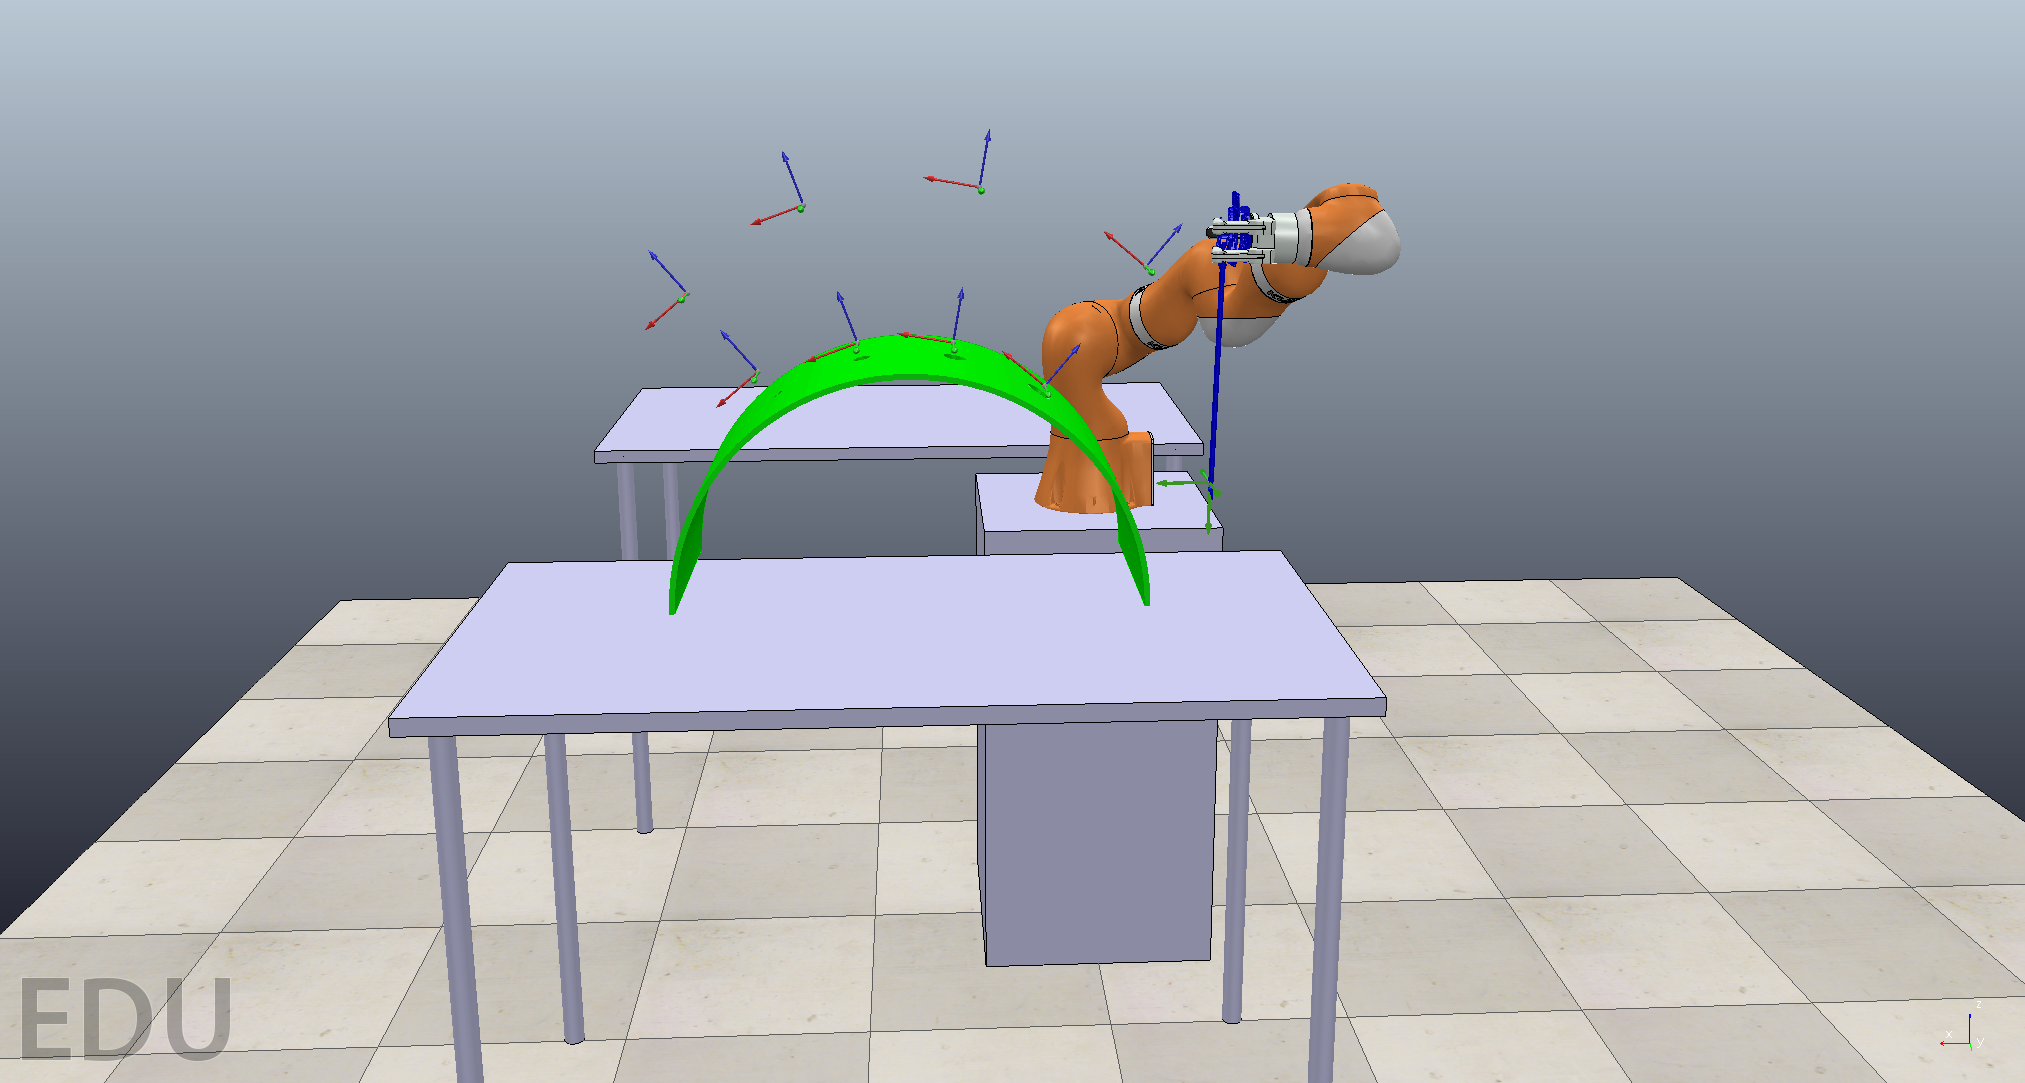
\includegraphics[width=\textwidth]{images/quick-vrep-prototyping.png}\\
\caption{Quick Prototyping using the VREP (CoppeliaSim) simulation environment}
\end{figure}
\end{center}